\section{Citation Fidelity}
\label{sec:citations}

The rubric used to grade \sys{} reports in \Cref{sec:experiments} scored claims with citations as supported, but did not check that the cited source actually made the claim. \citet{liu2023verifiability} found that around one quarter of the citations produced by generative search engines did not support their sentences. This section measures the citation fidelity of \sys{} reports. It first introduces an automatic test for checking citation fidelity, validates it on correctly-cited claims, and then applies it to all \sys{} reports to find where the link to sources is lost.

\subsection{A lexical attribution test}
The test exploits the intuition that a particular sentence in a report is likely to use some unusual words from its source. The test calculates for every sentence in a report that has a citation, the TF-IDF cosine similarity \citep{salton1988termweighting} of that sentence with each source in the document, and ranks the sources. It then assigns a percentile rank to each cited source based on its ranking (0 is the best match, 1 is the worst match).

If the citations are correct, the cited sources would tend to be highly ranked (low percentile) whereas if they were random, the percentile rank would be distributed uniformly between 0 and 1 (with median 0.5). We report the results as the median percentile rank of all cited sources and as the proportion of claims where the single best matching source is cited, compared to the chance expectation. The test is model-free and can run on all reports. Being lexical, the test risks under-ranking a source if it uses different wording, a practical limitation we measure in the validation.

A sensible validation is to ask whether the test can identify citations known to be correct. The leaf answers in the running log (\Cref{app:dag}) provide a ground truth by construction: each was generated by a single model call and the excerpts it cited were retrieved directly from the relevant documents. Against the set of all \atValMeanCandidates{} sources used by the run, the cited source is the best match for \atValBestCitedPct\% of leaf claims. (Note that a ratio of \atValBestChancePct\% is expected by chance.) The median percentile of the cited sources is 4\% (95\% confidence interval: [0\%, 8\%]).

Our evaluated reports cite full web pages, which means that a web page cited as a source also contains text unrelated to the claim. We repeated the validation test with the full text of each page. Against the \atValPagesMeanCandidates{} pages containing usable text, the best match is cited as source for \atValPagesBestCitedPct\% of claims, \atValPagesBestChancePct\% by chance. The test again distinguishes between correct citations and random ones.

\begin{table}[t]
\centering
\small
\resizebox{\linewidth}{!}{\begin{tabular}{lrrrrr}
\toprule
Setting & Claim--source pairs & Median rank percentile & Top-3 hit rate & Chance & Best match cited \\
\midrule
Leaf answers, own numbering & 63 & 0.04 [0.00, 0.08] & 0.83 & 0.12 & 0.96 (chance 0.10) \\
Leaf answers, own numbering, full pages & 24 & 0.00 [0.00, 0.11] & 0.88 & 0.30 & 0.84 (chance 0.13) \\
Leaf answers as a parent reads them, global numbering & 63 & 0.04 [0.00, 0.08] & 0.83 & 0.12 & 0.96 (chance 0.10) \\
Leaf answers as a parent read them, original pipeline & 63 & 0.12 [0.08, 0.16] & 0.49 & 0.12 & 0.52 (chance 0.10) \\
Final report, logged run & 173 & 0.48 [0.44, 0.52] & 0.06 & 0.12 & 0.04 (chance 0.10) \\
Evaluated reports, all listed sources & 491 & 0.47 [0.40, 0.53] & 0.18 & 0.14 & 0.14 (chance 0.10) \\
Evaluated reports, cited sources only & 491 & 0.43 [0.40, 0.50] & 0.56 & 0.51 & 0.41 (chance 0.36) \\
\bottomrule
\end{tabular}
}
\caption{Attributions of cited claims. Each row ranks all available sources according to the lexical similarity between their text and the text of each cited claim. The cited sources have median rank percentile 0 if always cited correctly, and 0.5 if citations are random (95\% bootstrap confidence interval in brackets). Top-3 hit rate is the fraction of cited sources that rank in the top 3. The column of chance values shows the top-3 hit rate expected under random citation. The final column shows the fraction of claims for which the best match was cited.}
\label{tab:attribution}
\end{table}

\begin{figure}[t]
\centering
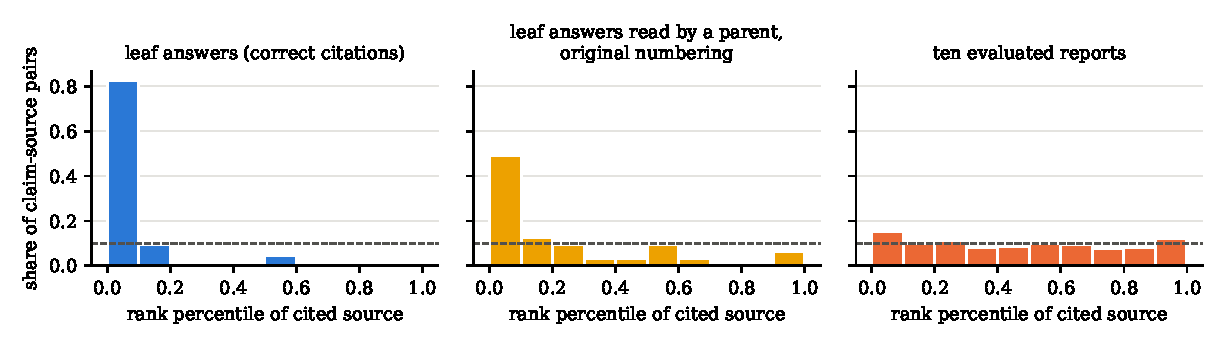
\includegraphics[width=\linewidth]{figs/attribution.pdf}
\caption{Rank percentiles of cited sources. If citations are correct, then they cluster around 0 on the left-hand side of the figure. In contrast, the distributions of percentiles of the evaluated reports' citations are flat as expected by random citation on the right-hand side. The middle panel shows the percentiles of the leaf answers as read by a parent node during composition, \Cref{sec:mechanism}. A dashed line indicates the uniform distribution.}
\label{fig:attribution}
\end{figure}

\subsection{Results}
\Cref{tab:attribution} and \Cref{fig:attribution} summarise the results. Our 10 evaluated reports contain \atEvalClaims{} citations of claims and \atEvalPairs{} (source, claim)-pairs. Against each report's listed sources, the median percentile of cited sources is \atEvalMedianPct{} (\atEvalPctLo{} to \atEvalPctHi), indistinguishable from the 0.5 expected under random citation. Against that same set, the best match is cited as source for \atEvalBestCitedPct\% of claims, by chance \atEvalBestChancePct\%. If we limit our comparison to the sources each report actually cites (a median of \atEvalCitedMeanCandidates{} per report), the picture does not change: the best match is cited as source for \atEvalCitedBestCitedPct\% of claims, by chance \atEvalCitedBestChancePct\%.

Finally, the last report produced by our logged run, which was produced using the same report-writing step, continues to perform at chance, with a median percentile of \atLogMedianPct. The information provided by the evaluated reports' citations is, in terms of our validation test, no more than random guesses about the source supporting each claim.

For instance, a bullet point stating that ``non-theistic systems such as Confucianism, Buddhism, and Stoicism achieved moral stability'' without divine law cites a collection of 5 sources that argue from the moral law for the existence of God. None of these sources are the origin of the claim. Similarly, a bullet point on ancient Egyptian, Israelite, and Vedic societies cites a work titled ``A Beginner's Guide to the Moral Argument''. While the claims may be correct, the citations are not.

\subsection{Mechanism}
\label{sec:mechanism}
The code for the evaluated reports is not available (\Cref{app:changes}). However, a snapshot of the repository, taken a week earlier, comes with a run that we have used above. We find that this snapshot of the system loses the link between claims and sources at two steps, both of which are consistent with the pattern we observed in the evaluated reports, though we cannot confirm them on the code we have for the evaluated system.

\paragraph{Local numbers read against a merged list.}
Each leaf answer numbers its own sources locally, as [1] through to [$k$]. When the parent of the leaf is composed, the pipeline merges the sources of its children into a single, deduplicated list, numbered [1] through to [$m$]. Then the synthesis model is instructed to cite these numbers from the merged list. When the children's answers are passed to the parent node, they retain their original local numbers. Thus, when the second child's answer contains ``[1]'' and that is copied into the parent, it is the first source from the first child in the merged list, not the first source from the second child. The central rows of \Cref{tab:attribution} demonstrate this step on our logged run.

Against the parent's merged list, the best match is cited for only \atOldBestCitedPct\% of leaf claims, mostly those taken from the first child of each parent. When we restore the leaf answers' local numbering, the \atOldBestCitedPct\% jumps back to \atValBestCitedPct\%. Since each level in the tree repeats this merge, the misattribution grows as answers propagate up the graph towards the root.

\paragraph{Node identifiers in place of sources.}
Note that the composition instructions for Phase 1 required each child to be cited by node identifier, so that downstream steps could track their dependencies. But the synthesis prompt asks the model to cite sources by number, which is how citations appear in the final report. (This is another conflict in instructions that should be addressed.) In the logged run, in which \dagParents{} nodes were composed, including the root, three of them, including the root, followed the composition instructions, writing source markers as ``(node\_3)'' with no source number. As a result, the report writer received a root answer without citations but with a command to number them, and it then assigned them arbitrarily. This explains why the final report in the logged run performed no better than chance.

\subsection{Correction}
This problem and the other one described in the preceding section can be solved by assigning a single, persistent identity to each source throughout the course of the run. In the corrected pipeline, each source is assigned a single global number the first time it is retrieved by any node. Leaf answers are translated from local identifiers to global numbers before being stored, so that all nodes in the run share the same numbering and the report's bibliography does too. After each composition, node identifiers are translated to global citations for the children in the parent answer, and any numbers not associated with the parent's sources are dropped. The synthesis and composition-instruction prompts are then modified to require citation by source number rather than node identifier.

If we replay the logged run with this correction, leaf claims are cited by their best matching source \atFixBestCitedPct\% of the time, just as in the leaf itself. (This study does not have any way to determine whether the attribution is preserved end to end through the report-writing step, and new experiments would be required to establish that, but the current tests make such a check inexpensive.)

\subsection{Implications}
Finally, the rate of supported claims in \Cref{tab:human} is computed by counting citation markers. This metric measures the frequency with which \sys{} adds citations, which it does more densely than STORM (\Cref{sec:analysis}), but it says nothing about whether the claims are actually supported by the cited sources. We should not assume that the reports are more ``grounded'' than the baselines on this basis. This test is easy to apply to any system that produces inline citations, but we were not able to apply it to either baseline, because the exports from STORM did not include URLs and Deep Research reports were not retained.
